%%%%%%%%%%%%%%%%%%%%%%%%%%%%%%%%%%%%%%%%%%%%%%%%%%%%%%%%%%%%%%%%%%% 
%                                                                 %
%                            CHAPTER                              %
%                                                                 %
%%%%%%%%%%%%%%%%%%%%%%%%%%%%%%%%%%%%%%%%%%%%%%%%%%%%%%%%%%%%%%%%%%% 
\chapter{Implementation}
\label{chapter:implementation}
In this chapter we present the design and implementation of the proposed system. The design and any of its components are not bound to any specific technology, as such they can be implemented using any programming language, framework or mapping language. For the implementation we first present the general setup of the environment. We then present the implementation of the data retrieval. Lastly we present some implementations of template creation and filling.

\section{System Design}
The system we propose is a pipeline that takes as input a knowledge graph and set of mapping rules and outputs the source files from which it would have been constructed. It has the advantage of being very modular, consisting of just data retrieval and template creation/filling. Depending on the mapping rules and config files different modules will be used. The graph source will decide the data retrieval strategy while the output file will determine the templating engine to be used. An overview of the design can be seen in figure \ref{fig:design}.

\begin{figure}
    \centering
    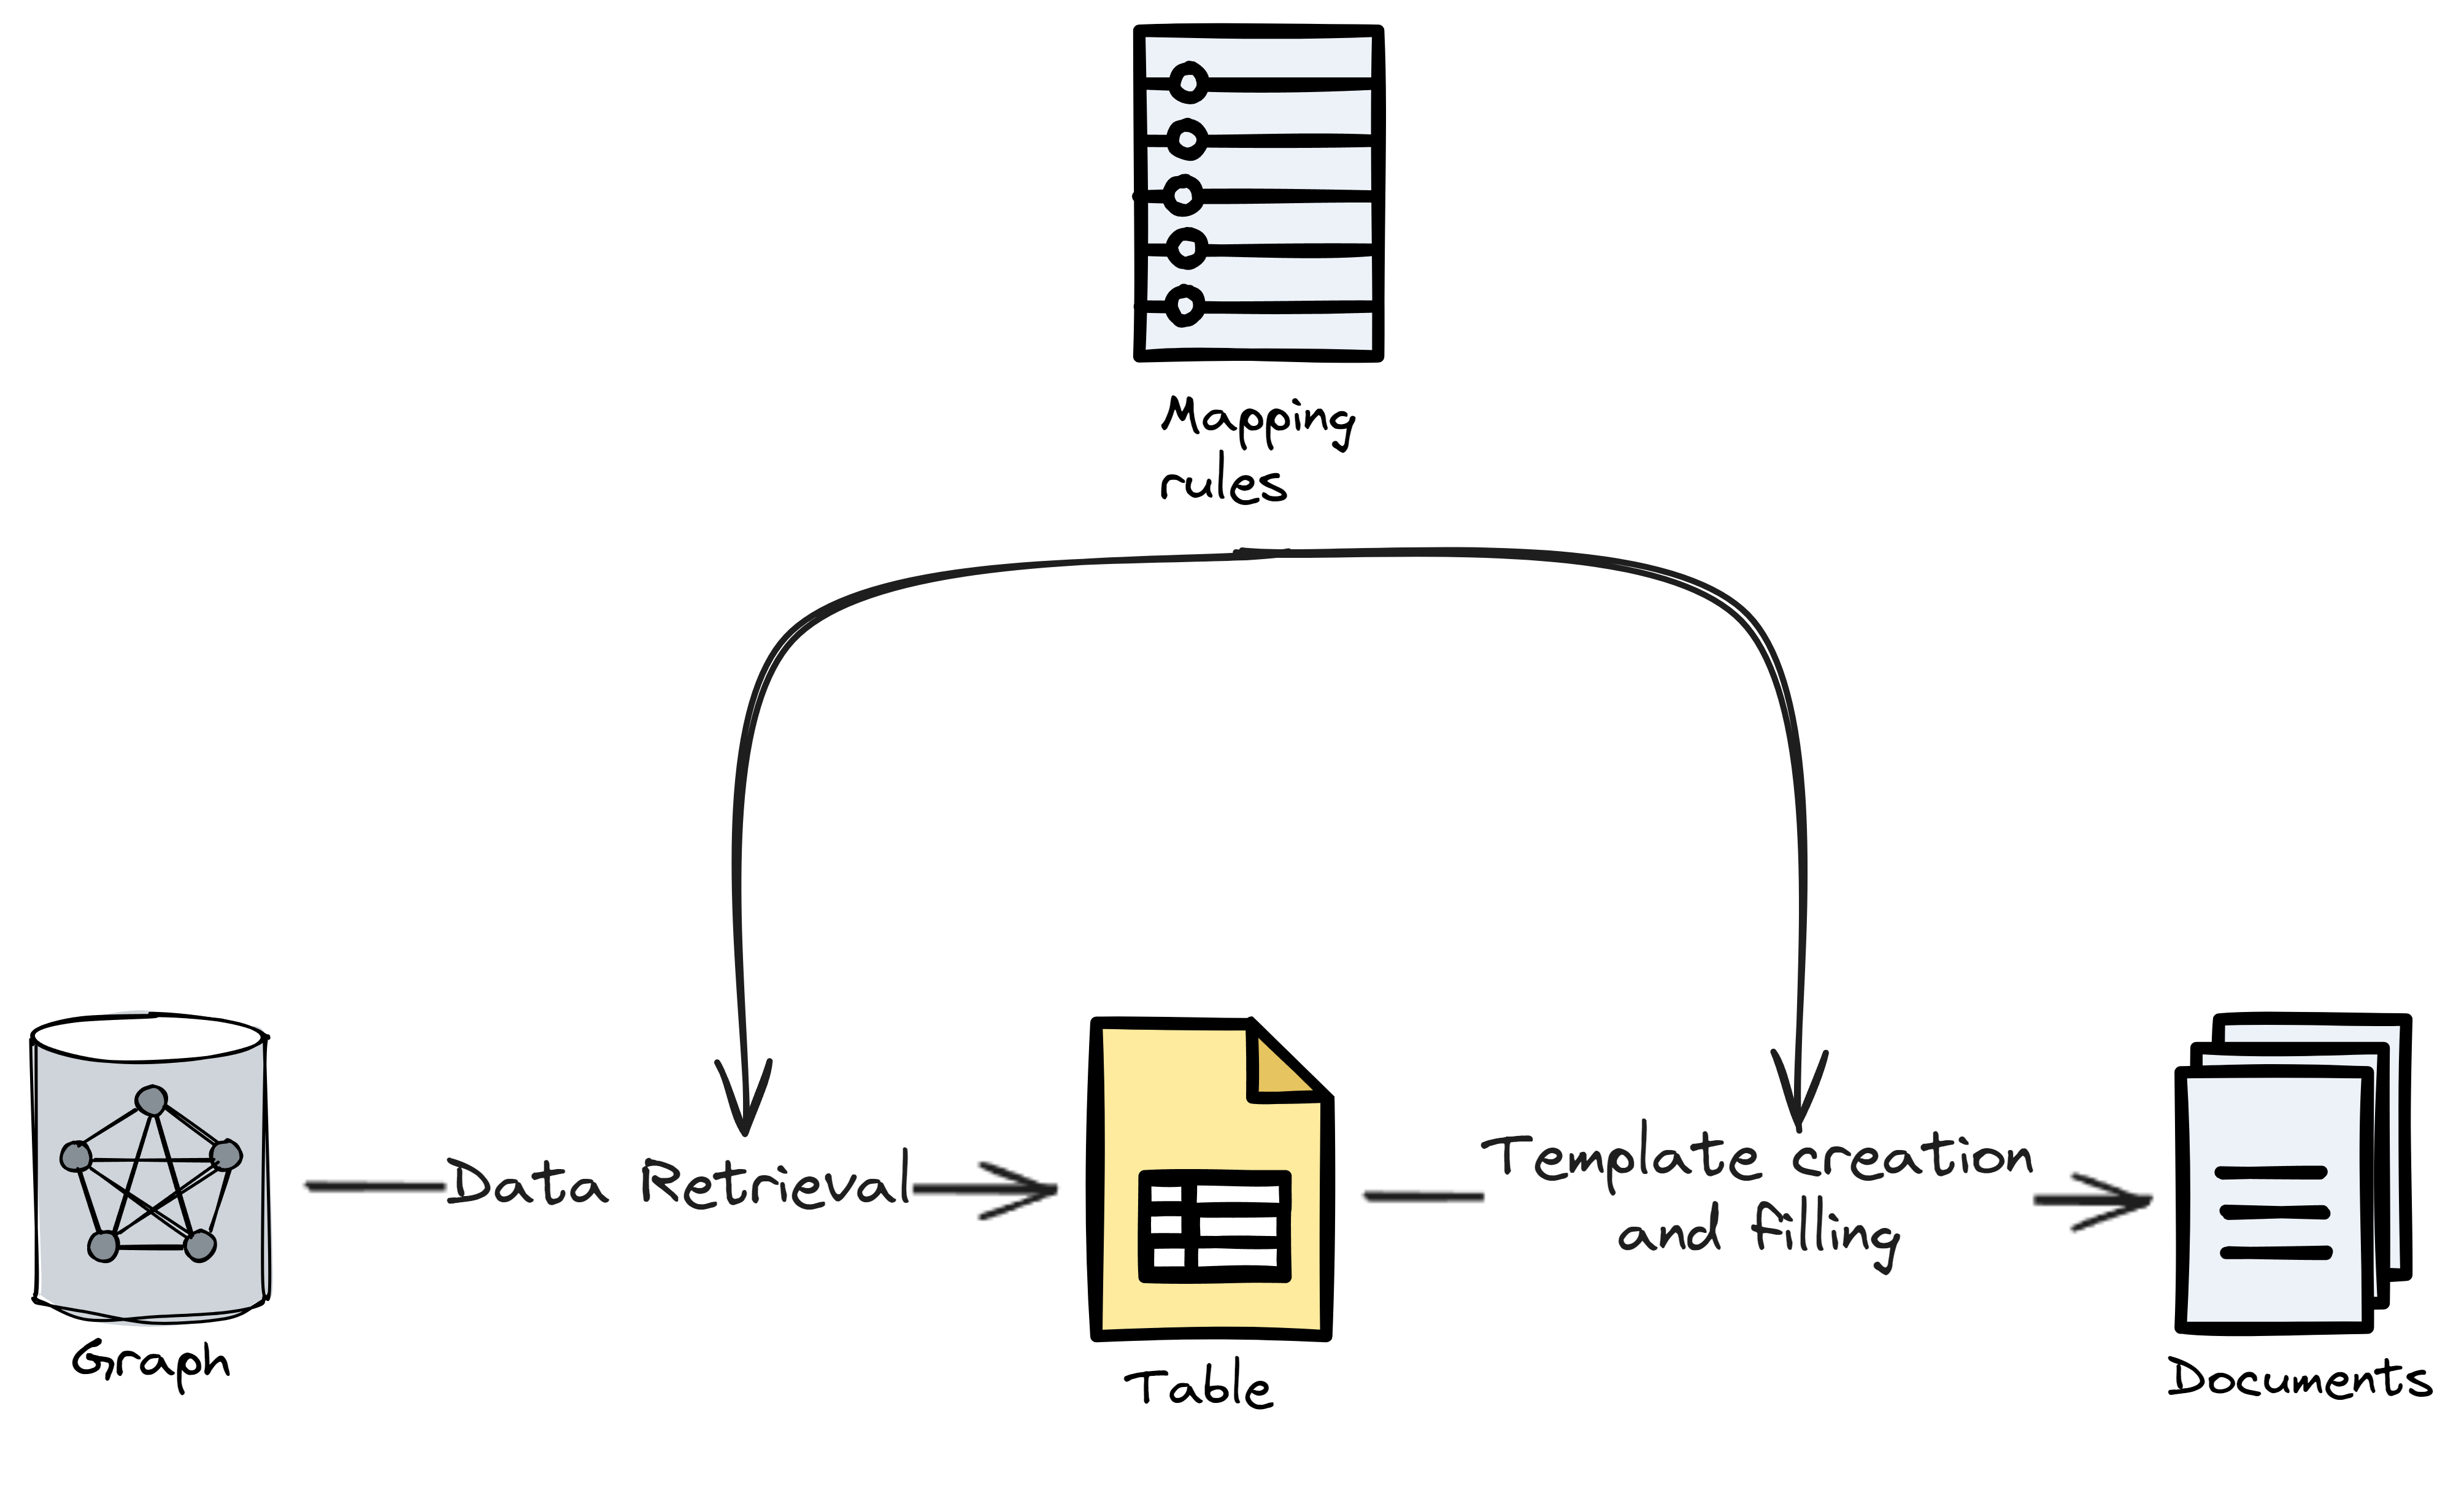
\includegraphics[width=0.9\textwidth]{fig/design.png}
    \caption{Design of the proposed system}
    \label{fig:design}   
\end{figure}


% At this time we only have a PoC implementation, as such many details haven't been worked out yet. For example, the section on creating the schema is limited, as we only handle CSV files which require little to no schema. 

\section{Setup}

We choose to make our implementation in Python as it both has an extensive set of libraries and is well suited for rapid development. We use Morph-KGC to process the mapping rules for its ease of use, being well made and its use of the pandas library to represent the mapping rules. As the graph source we choose a standalone SPARQL endpoint on a triple store. For working with graph(\acrshort{rdf}) files, we first upload them to a triple store.

First the endpoint is set up, if necessary. If the source is a file, it is uploaded to the endpoint using the SPARQL 1.1 Graph Store HTTP Protocol. In our setup this is a locally running the free version of GraphDB. The url of the repository is then wrapped using the SPARQLWrapper library and some settings are set.

Next we load the mapping rules from the mapping(\acrshort{rml}) files using Morph-KGC's internal \texttt{retrieve\_mappings} function. This function takes a config file (.ini format) as input, which specifies the location of the mapping files and various other settings which can be used to configure the behavior of the mapping. The mappings are returned as a pandas DataFrame which we enrich with various helper columns. An example of a single mapping rule (row in the DataFrame) can be found in listing \ref{lst:mapping_rule}. Marked in bold are the helper columns we add.

\begin{lstlisting}[caption={Example of a mapping rule in Morph-KGC}, label={lst:mapping_rule}, captionpos=b, basicstyle=\small]
source_name: DataSource1
triples_map_id: #TM0
triples_map_type: http://w3id.org/rml/TriplesMap
logical_source_type: http://w3id.org/rml/source
logical_source_value: student.csv
iterator: nan
subject_map_type: http://w3id.org/rml/template
subject_map_value: http://example.com/{Name}
[*subject_references_template: http://example.com/([^\/]*)$*]
[*subject_references: ['Name']*]
[*subject_reference_count: 1*]
subject_termtype: http://w3id.org/rml/IRI
predicate_map_type: http://w3id.org/rml/constant
predicate_map_value: http://xmlns.com/foaf/0.1/name
[*predicate_references_template: None
predicate_references: []
predicate_reference_count: 0*]
object_map_type: http://w3id.org/rml/reference
object_map_value: Name
[*object_references_template: None
object_references: ['Name']
object_reference_count: 1*]
object_termtype: http://w3id.org/rml/Literal
object_datatype: nan
object_language: nan
graph_map_type: http://w3id.org/rml/constant
graph_map_value: http://w3id.org/rml/defaultGraph
subject_join_conditions: nan
object_join_conditions: nan
source_type: CSV
mapping_partition: 1-1-1-1
\end{lstlisting}

\section{Retrieving the data}
\label{section:retrieving_data}
Retrieving the data is done by querying the \acrshort{sparql} endpoint using an automatically generated query. All the required data from the source is retrieved at once. This does result in some degree of duplication for nested structures, but doing all processing and joining server-side is preferable. This also has a disadvantage in disjointed mappings resulting in a Cartesian product of the fragments. This is further discussed in subsection \ref{subsection:disjointed_mappings}. The data is returned as a CSV-table which is then loaded into a pandas DataFrame for further processing. The only post processing done at the moment is the decoding of url-encoded strings where necessary. 

\subsection{Generating the queries}
\label{subsection:generating_queries}
To generate the queries we first select the triple maps we want to use to generate the query. While constant values are always included, sometimes we can lighten the load on the server by reducing the amount and complexity of mapping rules we use. We design three operating modes:
\begin{itemize}
    \item \textbf{Full}: All triple maps are used to generate the query. This is guaranteed to give predicatable results as it checks each instance of a mapped value.
    \item \textbf{Reduced}: All triple maps with a object map type of reference are used to generate the query. Only where necessary to retrieve all data template map types are used.
    \item \textbf{Minimal}: Only a single datapoint is used for each reference, with a preference for reference object map types.
\end{itemize}

We then generate the queries by translating the mapping rules into patterns. 
Each of the three map types, constant, reference, and template, generates a different pattern.
For the constant map type, we know that it will always be present with a constant value, so we can simply add it as a triple pattern like \texttt{?s a foaf:Person .}. 
Both reference and template map types will not generate a triple during materialization if any of the references are not present during the generation. We must take this into account by allowing for blank fields using the optional keyword.
Reference maps are the easiest to work with as they directly translate back to the source. An example of a basic query using constant and reference maps can be found in listing \ref{lst:simple_query_example}.

\begin{lstlisting}[caption={Simple query example}, label={lst:simple_query_example}, captionpos=b]
SELECT DISTINCT ?Name ?ID
WHERE {
    ?s a foaf:Person .

    optional{
        ?s foaf:name ?Name .
    }
    optional{
        ?s ex:id ?ID .
    }
}
\end{lstlisting}    

Template maps are the most complex to work with as their structure can wildly vary. The simplest step we can take is to confirm the mapped value matches with the map template like
\texttt{FILTER(regex(str(?s), "http://example.com/([\textasciicircum\textbackslash\textbackslash/]*)/([\textasciicircum\textbackslash\textbackslash/]*)\$"))}. Taking this further we can use string manipulation to split the variable into the different references. An example of this can be found in listing \ref{lst:template_query_example}.

\begin{lstlisting}[caption={Template query example}, label={lst:template_query_example}, captionpos=b]
SELECT DISTINCT ?Name ?ID
WHERE {
    ?s a foaf:Person .
    FILTER(regex(str(?s), "http://example\\.com/([^\\/]*)/([^\\/]*)$")) .
    BIND(STRAFTER(str(?s), "http://example.com/") as ?temp) .
    BIND(STRBEFORE(str(?temp), "/") as ?ID)
    BIND(STRAFTER(?temp, "/") as ?Name)

    optional{
        ?s foaf:name ?Name .
    }
    optional{
        ?s ex:id ?ID .
    }
}
\end{lstlisting}

The algorithm for generating the queries can be found in algorithm \ref{alg:generate_query}. This is still an early version of the algorithm, which needs to be improved to handle more complex mappings.

\begin{algorithm} 
    \caption{Generating the queries}
    \label{alg:generate_query}
    \begin{algorithmic}[1]
        \Require{$iterator$ is the iterator to generate the query for}
        \Require{$mapping\_rules$ is a set of mapping rules for said iterator}
        \State $query\_lines \gets []$
        \ForAll{$rule \in mapping\_rules$}
            \If{$rule.is\_constant()$}
                \State $query\_lines.append(rule.to\_triple())$ 
            \ElsIf{$rule.is\_reference()$}
                \State $query\_lines.append(rule.to\_optional\_triple())$
            \ElsIf{$rule.is\_template()$}
                \State $query\_lines.append(test\_object\_regex(rule))$
                \State $remainder \gets rule['object\_map\_value']$
                \ForAll{$reference \in rule['object\_references']$}
                    \State $query\_lines.append(bind_reference_part(rule, reference))$
                \EndFor
            \EndIf
        \EndFor
        \State $query \gets wrap\_query\_lines(query\_lines)$
    \end{algorithmic}
\end{algorithm}

\subsection{Disjointed mappings}
\label{subsection:disjointed_mappings}

We generate a single query for each iterator. This query can contain multiple subjects. This can, however, lead to issues when the subjects share no references. The effect we get is not unlike joining two tables in SQL without join conditions. For example, using the mapping listed in listing \ref{lst:bad_join_example} we get the query in listing \ref{lst:bad_join_query}. When applied to the knowledge graph in listing \ref{lst:bad_join_kg} we get the result in listing \ref{lst:bad_join_result} instead of the original source in listing \ref{lst:bad_join_expected_result}. When converting the badly generated source back to the knowledge graph, we do get the same knowledge graph as the original as the duplicate data is ignored. The amount of duplicate data increases exponentially with the number of subjects so even though ignoring it would be a valid solution, it is not viable with larger datasets. The only solution to this problem is updating the mapping rules to either split the source or add shared references. The user is ultimately responsible for this, but we could generate a warning to notify the user. 

\begin{listing}
    \refstepcounter{lstlisting}
    \noindent\begin{minipage}[b]{.45\textwidth}
        \begin{lstlisting}[basicstyle=\small]
<TriplesMap1> a rr:TriplesMap;
rml:logicalSource [ 
    rml:source "student_sport.csv";
    rml:referenceFormulation ql:CSV
];
rr:subjectMap [ 
    rr:template "http://example.com/{Student}";
    rr:class ex:Student
];
rr:predicateObjectMap [ 
    rr:predicate foaf:name ; 
    rr:objectMap [ 
        rml:reference "Student"
    ]
].
        \end{lstlisting}      
    \end{minipage}
    \hfill
    \begin{minipage}[b]{.45\textwidth}
        \begin{lstlisting}[basicstyle=\small]
<TriplesMap2> a rr:TriplesMap;
rml:logicalSource [ 
    rml:source "student_sport.csv";
    rml:referenceFormulation ql:CSV
];
rr:subjectMap [ 
    rr:template "http://example.com/{Sport}";
    rr:class ex:Sport
];
rr:predicateObjectMap [ 
    rr:predicate foaf:name ; 
    rr:objectMap [ 
        rml:reference "Sport"
    ]
].
        \end{lstlisting}
    \end{minipage}
    \addtocounter{listing}{5}
    \caption{Bad join mapping}
    \label{lst:bad_join_example}
\end{listing}

\begin{lstlisting}[caption={Bad join query (trimmed)}, label={lst:bad_join_query}, captionpos=b, basicstyle=\small]






SELECT DISTINCT ?Student_name ?Sport
WHERE {
    ?s1 a ex:Student .
    optional{
        ?s1 foaf:name ?Student_name .
    }
    ?s2 a ex:Sport .
    optional{
        ?s2 foaf:name ?Sport .
    }
}
\end{lstlisting}

\begin{lstlisting}[caption={Bad join knowledge graph}, label={lst:bad_join_kg}, captionpos=b, basicstyle=\small]
@prefix ex: <http://example.com/> .
@prefix foaf: <http://xmlns.com/foaf/0.1/> .

ex:Venus a ex:Student ;
    foaf:name "Venus" .
ex:Tom a ex:Student ;
    foaf:name "Tom" .
ex:Tennis a ex:Sport ;
    foaf:name "Tennis" .
ex:Football a ex:Sport ;
    foaf:name "Football" .
\end{lstlisting}

\begin{lstlisting}[caption={Bad join result}, label={lst:bad_join_result}, captionpos=b, basicstyle=\small]
Student,Sport
Venus,Tennis
Venus,Football
Tom,Tennis
Tom,Football
\end{lstlisting}

\begin{lstlisting}[caption={Bad join original source}, label={lst:bad_join_expected_result}, captionpos=b]
Student,Sport
Venus,Tennis
Tom,Football
\end{lstlisting}

\section{Contructing the schema}
\label{section:constructing_schema}
Constructing the schema is done by reversing the mapping rules' source. We do this using the iterator and the mapping rule's references. \acrshort{rml} supports many different types of sources and referenceFormulations. We will implement the CSV, xPath, and JSONPath referenceFormulations. Not every source is a file, so for query-based sources, we will generate the query output. In a later stage, we could look into taking it a step further, generating the actual source behind those intermediate results.

As each referenceFormulation has its reference syntax, we will have to tailor the implementation to each referenceFormulation. For the PoC, we only implement the CSV referenceFormulation. 

\subsection{CSV}
\label{subsection:csv}
The CSV referenceFormulation is the simplest of the three as it describes a simple two-dimensional table, with columns having the names of the references and rows being the iterated values. The example TriplesMap in listing \ref{lst:csv_file_mapping} results in the CSV template in listing \ref{lst:csv_file}. Unlike the other referenceFormulations, CSV has no uncertainty in terms of structure.

\begin{lstlisting}[caption={Example mapping for a CSV file}, label={lst:csv_file_mapping}, captionpos=b, basicstyle=\small]
<TriplesMap1> a rr:TriplesMap;

rml:logicalSource [ 
    rml:source "student.csv";
    rml:referenceFormulation ql:CSV
];

rr:subjectMap [ 
    rr:template "http://example.com/Student/{ID}/{Name}";
    rr:graph ex:PersonGraph ;
    rr:class foaf:Person
];

rr:predicateObjectMap [ 
    rr:predicate ex:id ; 
    rr:objectMap [ rml:reference "ID" ]
];

rr:predicateObjectMap [ 
    rr:predicate foaf:name ; 
    rr:objectMap [ rml:reference "Name" ]
].
\end{lstlisting}

\begin{lstlisting}[caption={Example CSV template}, label={lst:csv_file}, captionpos=b, basicstyle=\small]
[*ID,Name*]
<ID>,<Name>
\end{lstlisting}

\section{Applying the data to the schema}
\label{section:applying_data}
Generating the final output is done by iterating over the rows of the data and applying them to the schema. Each column of the data corresponds to a reference in the schema. A short version of the algorithm can be found in algorithm \ref{alg:apply_data}. For the PoC this approach is sufficient, even too complex as we can simply dump the query-result DataFrame to a CSV file. For more complex, possibly nested, sources we will have to adapt this algorithm.

\begin{algorithm}
    \caption{Applying the data to a simple (non-nested) schema}
    \label{alg:apply_data}
    \begin{algorithmic}[1]
        \Require{$schema$ is a schema}
        \Require{$data$ is a DataFrame}
        \State $output \gets new\_file$
        \ForAll{$row \in data$}
            \State $output \gets schema$
            \ForAll{$column \in row$}
                \State $schema.replace(column.name, column.value)$
            \EndFor
            \State $output.write(schema)$
        \EndFor
    \end{algorithmic}
\end{algorithm}
